\documentclass[aspectratio=169,11pt]{beamer}

% ============================================================
% A Tiered Compilation Architecture for Low-Latency Wasm
% Runtimes in Edge Computing Environments
% Master's Thesis Defense -- Hsiang-Yu Lee (NTU CSIE)
% ============================================================

\usepackage{fontspec}
\usepackage{xeCJK}
\IfFontExistsTF{Noto Sans CJK TC}{\setCJKmainfont{Noto Sans CJK TC}}{%
  \IfFontExistsTF{Noto Sans CJK SC}{\setCJKmainfont{Noto Sans CJK SC}}{%
    \IfFontExistsTF{WenQuanYi Zen Hei}{\setCJKmainfont{WenQuanYi Zen Hei}}{}}}
\usepackage{lmodern}
\usepackage{booktabs}
\usepackage{array}
\usepackage{tikz}
\usepackage{listings}
\usepackage{xcolor}
\usepackage{amsmath}
\usepackage{calc}

\usetikzlibrary{shapes.geometric,arrows.meta,positioning,fit,backgrounds,calc}

\IfFileExists{beamerthememetropolis.sty}{%
  \usetheme{metropolis}
  \metroset{progressbar=frametitle,numbering=fraction,block=fill}
}{%
  \usetheme{Madrid}
  \usecolortheme{seahorse}
}

\definecolor{nturoyal}{HTML}{1B4F8C}
\definecolor{ntugold}{HTML}{C8A951}
\definecolor{tier1}{HTML}{4E79A7}
\definecolor{tier2}{HTML}{E15759}
\definecolor{osrcol}{HTML}{59A14F}
\definecolor{neutral}{HTML}{555555}
\setbeamercolor{frametitle}{bg=nturoyal,fg=white}

\lstset{
  basicstyle=\ttfamily\scriptsize,
  keywordstyle=\color{nturoyal}\bfseries,
  commentstyle=\color{neutral}\itshape,
  numbers=none,
  showstringspaces=false,
  breaklines=true,
  frame=single,
  framerule=0pt,
  backgroundcolor=\color{black!4},
  xleftmargin=4pt,xrightmargin=4pt,
}

\newcommand{\tone}{\textbf{\textcolor{tier1}{Tier-1}}}
\newcommand{\ttwo}{\textbf{\textcolor{tier2}{Tier-2}}}
\newcommand{\osr}{\textbf{\textcolor{osrcol}{OSR}}}
\newcommand{\code}[1]{{\ttfamily\small #1}}

\title[Tiered Wasm Compilation]{A Tiered Compilation Architecture for\\Low-Latency Wasm Runtimes in Edge Computing}
\subtitle{Master's Thesis Defense}
\author[Hsiang-Yu Lee]{Hsiang-Yu Lee\,(李祥宇)\\\small Advisor: Prof.\ Shih-Wei Liao}
\institute[NTU CSIE]{Department of Computer Science and Information Engineering\\National Taiwan University}
\date{May 22, 2026}

\begin{document}

% ------------------------------------------------------------
\begin{frame}[plain]
  \titlepage
\end{frame}

\begin{frame}{Outline}
  \tableofcontents
\end{frame}

% ============================================================
\section{Motivation}
% ============================================================

\begin{frame}{Edge computing reshapes the workload}
  \begin{columns}[T,onlytextwidth]
    \begin{column}{0.55\textwidth}
      \textbf{Edge nodes face two tight budgets.}
      \begin{itemize}\setlength{\itemsep}{2pt}
        \item \textbf{Response time:} tens of milliseconds per request.
        \item \textbf{Resources:} 1--2\,GB RAM and few vCPUs.
      \end{itemize}
      \vspace{0.5em}
      The workload mix is short-lived, stateless functions that start and exit constantly.
      \vspace{0.7em}

      \textbf{WebAssembly fits the role.}
      The format is compact, language-agnostic, sandboxed, and predictable.
      Fastly Compute, Cloudflare Workers, and Fermyon Spin all run WebAssembly in production.
    \end{column}
    \begin{column}{0.42\textwidth}
      \centering
      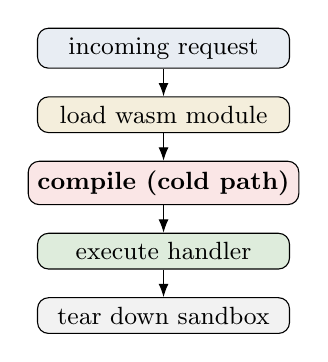
\begin{tikzpicture}[node distance=3.5mm, every node/.style={font=\small}]
        \node[draw,rounded corners,fill=nturoyal!10,minimum width=3.2cm] (req)  {incoming request};
        \node[draw,rounded corners,fill=ntugold!20,minimum width=3.2cm,below=of req] (load) {load wasm module};
        \node[draw,rounded corners,fill=tier2!15,minimum width=3.2cm,below=of load] (comp) {\textbf{compile (cold path)}};
        \node[draw,rounded corners,fill=osrcol!20,minimum width=3.2cm,below=of comp] (exec) {execute handler};
        \node[draw,rounded corners,fill=black!5,minimum width=3.2cm,below=of exec] (tear) {tear down sandbox};
        \draw[-{Latex}] (req)--(load);
        \draw[-{Latex}] (load)--(comp);
        \draw[-{Latex}] (comp)--(exec);
        \draw[-{Latex}] (exec)--(tear);
      \end{tikzpicture}\\[2pt]
      \scriptsize Per-request lifecycle.
    \end{column}
  \end{columns}
\end{frame}

% ============================================================
\begin{frame}{The WasmEdge cold-start bottleneck}
  WasmEdge is the leading server-side Wasm runtime.
  Microsoft, ByteDance, and Sony all run WasmEdge in production.

  \vspace{0.4em}
  \textbf{WasmEdge compiles with LLVM end-to-end.}
  The LLVM pipeline produces near-native code.
  The pipeline is also expensive:
  \begin{itemize}\setlength{\itemsep}{2pt}
    \item Compile time grows faster than module size.
    \item Memory usage during compilation is large.
    \item Every cold start pays the full compile cost.
  \end{itemize}

  \vspace{0.4em}
  \textbf{The structural problem.}
  A single-tier compiler treats every invocation the same way.
  A request that runs for one microsecond pays the same compile cost as one that runs for one minute.

\end{frame}

% ============================================================
\begin{frame}{Cold-start latency}
  \begin{block}{Definition}
    Time from request arrival to the first machine-code instruction of the requested wasm function. Assumes no ready-to-run compiled instance of the module is resident.
  \end{block}

  \vspace{0.3em}
  \begin{columns}[T,onlytextwidth]
    \begin{column}{0.48\textwidth}
      \textbf{Inside the window}
      \begin{itemize}\setlength{\itemsep}{1pt}
        \item load, parse, validate
        \item compile
        \item instantiate
      \end{itemize}
    \end{column}
    \begin{column}{0.48\textwidth}
      \textbf{Outside the window}
      \begin{itemize}\setlength{\itemsep}{1pt}
        \item the wasm function's own execution
        \item reported as steady-state work
      \end{itemize}
    \end{column}
  \end{columns}

\end{frame}

% ============================================================
\begin{frame}{Execution time is highly skewed}
  A small fraction of functions accounts for the bulk of run-time.
  \vspace{0.3em}
  \begin{itemize}\setlength{\itemsep}{2pt}
    \item Heavy optimization on cold functions wastes the compile budget.
    \item Cold functions receive optimization they do not need.
    \item Hot functions wait behind cold compilation before they can start.
  \end{itemize}
  \vspace{0.7em}
  \textbf{The established solution is tiered compilation.}
  \begin{itemize}\setlength{\itemsep}{2pt}
    \item A \tone{} baseline compiles every function fast.
    \item A \ttwo{} optimizer recompiles hot functions later, guided by profile data.
    \item V8, JavaScriptCore, and SpiderMonkey all use this pattern.
  \end{itemize}
  \vspace{0.5em}
  \alert{WasmEdge has no baseline tier, no profile-driven promotion, and no mid-execution code replacement.}
\end{frame}

% ============================================================
\begin{frame}{Related work}
  \small
  \textbf{Browser-engine Wasm pipelines.}
  V8 pairs Liftoff and TurboFan. JavaScriptCore runs IPInt, BBQ, and OMG. SpiderMonkey runs Baseline and Ion.
  All three use function-entry promotion.
  Public documentation reports no OSR between the baseline JIT and the optimizing JIT.

  \vspace{0.4em}
  \textbf{Server-side Wasm pipelines.}
  Wasmtime offers Cranelift (optimizing) and Winch (baseline).
  The runtime does not currently tier up between them.

  \vspace{0.4em}
  \textbf{OSR in language VMs.}
  HotSpot has supported OSR for over two decades.
  .NET 7 added OSR in 2022 with the one-shot-caller motivation this thesis also targets.
  Tracing JITs (PyPy, LuaJIT) sidestep OSR through trace recording.

  \vspace{0.4em}
  \alert{This thesis fills a gap.
  No published server-side WebAssembly runtime combines a non-LLVM Sea-of-Nodes baseline, selective LLVM-frontend reuse, and loop-level OSR.}
\end{frame}

% ============================================================
\section{Problem Statement and Contributions}
% ============================================================

\begin{frame}{Three sub-problems}
  \textbf{Goal.}
  Cut cold-start latency without giving up the steady-state throughput that LLVM delivers on hot code.
  \vspace{0.4em}
  \begin{description}\setlength{\itemsep}{0.5em}
    \item[\tone{} baseline.]
      Compile every wasm function fast at module load.
      Cover the full WebAssembly instruction set the workloads use.
      Reuse the existing WasmEdge runtime contracts.
    \item[\ttwo{} optimizer.]
      Reuse the LLVM frontend to recompile hot functions.
      Bridge the two tiers' calling conventions.
      Hide the LLVM compile cost from the user thread.
    \item[In-flight migration.]
      A function called once spends its run-time inside one long loop.
      The prologue never re-fires, so entry-table promotion delivers no speedup.
      A separate mechanism must migrate the running frame mid-loop.
  \end{description}
\end{frame}

% ============================================================
\begin{frame}{Contributions}
  \small
  \begin{enumerate}\setlength{\itemsep}{0.5em}
    \item \textbf{\tone{} baseline JIT for WasmEdge.}\\
      Integrate a lightweight Sea-of-Nodes library.\\
      Translate wasm bytecode to sea-of-nodes IR nodes.\\
      Embed per-function and per-loop profile counters directly in compiled code.
    \item \textbf{\ttwo{} selective LLVM-frontend recompilation.}\\
      Design a heuristic to synthesizes a mini-module per batch.\\
      Design three ABI bridge thunks to bridge the calling convention gap between the 2 tiers.
    \item \textbf{On-Stack Replacement.}\\
      Instrument every outermost loop with a three-state back-edge diamond.\\
      Synthesize a continuation that starts execution at the loop header.
    \item \textbf{Empirical evaluation.}\\
      Report and discuss a step-by-step experiment on 39 strengthened sightglass kernels.
  \end{enumerate}
\end{frame}

% ============================================================
\section{Architecture Overview}
% ============================================================

\begin{frame}{System architecture}
  \vspace{4mm}
  \centering
  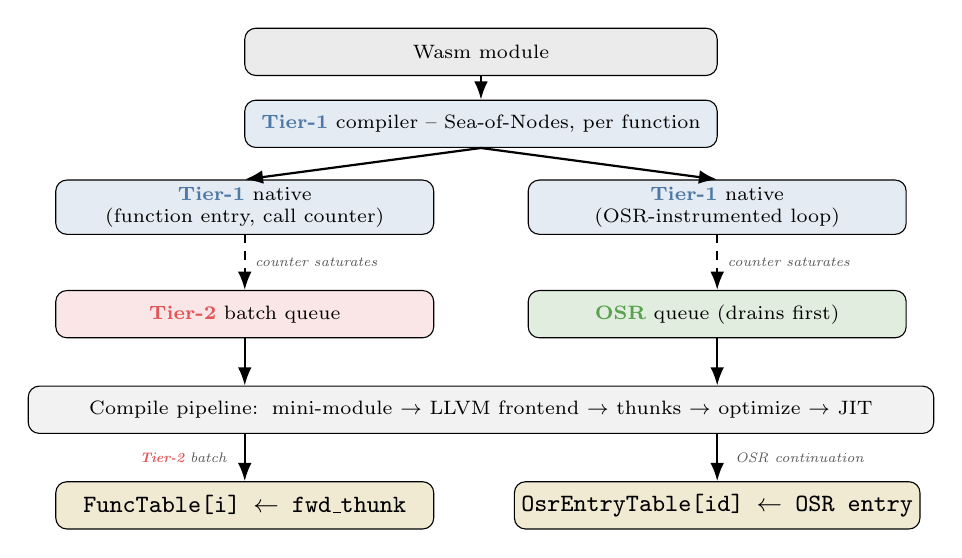
\begin{tikzpicture}[
    font=\scriptsize,
    box/.style={draw,rounded corners,minimum height=6mm,inner sep=2.5pt,align=center},
    t1/.style={box,fill=tier1!15},
    t2/.style={box,fill=tier2!15},
    osrb/.style={box,fill=osrcol!18},
    publ/.style={box,fill=ntugold!25},
    note/.style={font=\tiny\itshape,color=neutral},
    arr/.style={-{Latex},thick},
  ]
    \node[box,fill=black!8,minimum width=6cm] (mod) {Wasm module};
    \node[t1,below=3mm of mod,minimum width=6cm] (comp1) {\tone{} compiler -- Sea-of-Nodes, per function};
    \node[t1,below=4mm of comp1,xshift=-3cm,minimum width=4.8cm] (entry) {\tone{} native\\(function entry, call counter)};
    \node[t1,below=4mm of comp1,xshift=3cm,minimum width=4.8cm] (loop)  {\tone{} native\\(OSR-instrumented loop)};
    \node[t2,below=7mm of entry,minimum width=4.8cm] (batchq) {\ttwo{} batch queue};
    \node[osrb,below=7mm of loop,minimum width=4.8cm] (osrq) {\osr{} queue (drains first)};
    \node[box,fill=black!5,below=6mm of batchq.south,xshift=3cm,minimum width=11.5cm] (pipe)
      {Compile pipeline:\, mini-module $\to$ LLVM frontend $\to$ thunks $\to$ optimize $\to$ JIT};
    \node[publ,below=6mm of pipe,xshift=-3cm,minimum width=4.8cm] (ft)  {\code{FuncTable[i] $\leftarrow$ fwd\_thunk}};
    \node[publ,below=6mm of pipe,xshift=3cm,minimum width=4.8cm] (osrt) {\code{OsrEntryTable[id] $\leftarrow$ OSR entry}};

    \draw[arr] (mod) -- (comp1);
    \draw[arr] (comp1.south) -- (entry.north);
    \draw[arr] (comp1.south) -- (loop.north);
    \draw[arr,dashed] (entry) -- node[right,note]{counter saturates} (batchq);
    \draw[arr,dashed] (loop)  -- node[right,note]{counter saturates} (osrq);
    \draw[arr] (batchq.south) -- (pipe.north -| batchq.south);
    \draw[arr] (osrq.south)   -- (pipe.north -| osrq.south);
    \draw[arr] (pipe.south -| ft.north) -- node[left,note,xshift=-1mm]{\ttwo{} batch} (ft.north);
    \draw[arr] (pipe.south -| osrt.north) -- node[right,note,xshift=1mm]{OSR continuation} (osrt.north);
  \end{tikzpicture}
\end{frame}

\begin{frame}{Pipeline at a glance}
  \begin{itemize}\setlength{\itemsep}{4pt}
    \item The user thread runs \tone{} native code and trips the embedded counters.
    \item A heuristic selects a batch of functions to promote to \ttwo{} and synthesizes a mini-module for the batch.
    \item Two promotion paths feed two queues: function-entry promotion and loop OSR.
    \item A worker thread compiles \ttwo{} batches and OSR continuations in the background.
    %\item The worker drains the OSR queue first, as an OSR continuation must publish before the running loop exits.
    \item The worker publishes each result with one atomic store into the dispatch slot.
    %\item The pipeline coexists with the existing LLVM AOT path. Modules already compiled ahead of time skip \tone{}.
  \end{itemize}
\end{frame}

% ============================================================
\section{Tier-1: Baseline JIT}
% ============================================================

\begin{frame}{Tier-1: a lightweight Sea-of-Nodes baseline}
  \textbf{Code generator: dstogov/ir.}
  A small Sea-of-Nodes JIT library, descended from the Zend JIT in PHP 8.
  \begin{itemize}\setlength{\itemsep}{1pt}
    \item The library runs a fixed, linear pipeline. No pass manager.
    \item Compile latency stays bounded and predictable.
    \item The codebase is small enough to vendor and modify.
  \end{itemize}
  \vspace{0.5em}
  \textbf{Advantages of sea-of-nodes IR.}
  \begin{itemize}\setlength{\itemsep}{1pt}
    \item \textbf{SSA by construction.} Values are graph nodes. Definitions and uses are explicit edges. No separate SSA-construction phase.
    \item \textbf{One graph for control flow and data.} A single traversal covers both. Passes do not need parallel analyses.
    \item \textbf{Cheap global code motion.} Floating nodes let the scheduler choose placement after optimization.
    %\item \textbf{Dead code is implicit.} Unreachable nodes are never scheduled. No explicit DCE pass is required.
  \end{itemize}
\end{frame}

% ============================================================
\begin{frame}{Calling convention and \texttt{JitExecEnv}}
  \small
  \textbf{Every \tone{} function takes the same two arguments.}
  \[
    f(\texttt{env}^{*},~\texttt{args}^{*}) \to \texttt{void}
  \]
  The args buffer holds one 64-bit slot per wasm parameter.
  One dispatch shape covers wasm-defined functions, host imports, and indirect calls.

  \vspace{0.4em}
  \textbf{The \code{JitExecEnv} struct groups state into three sets.}
  \begin{center}
  \scriptsize
  \begin{tabular}{ll}
    \toprule
    Group & Contents \\
    \midrule
    Lookup tables    & \code{FuncTable}, linear memory, globals, indirect-call shadow \\
    Helper addresses & host call, memory growth, profile-saturation helpers \\
    Promotion state  & call counters, back-edge counters, \code{OsrEntryTable}, OSR buffer \\
    \bottomrule
  \end{tabular}
  \end{center}
  \vspace{0.2em}
  \scriptsize \code{JitExecEnv} points to shared tables; \ttwo{} publication updates \code{FuncTable} slots or \code{OsrEntryTable} slots.
\end{frame}

% ============================================================
\section{Tier-2: Selective LLVM Recompilation}
% ============================================================
\begin{frame}{Batch composition: walk up, then bounded BFS}
  \textbf{Promoting only the threshold-tripping function is not enough.}
  The function that trips the counter is often a small leaf inside a larger hot caller.
  A leaf promoted alone leaves its caller in \tone{}, so the optimizer cannot inline across the boundary.
  \vspace{0.3em}
  \begin{block}{Algorithm 2}
    \begin{enumerate}\setlength{\itemsep}{1pt}
      \item \textbf{Walk up one hop.} Pick the hottest direct caller as the batch root.
      \item \textbf{Bounded BFS.} Traverse direct callees from the root up to a depth limit and a batch size limit.
      \item \textbf{Two-test admission} for each candidate callee:
        \begin{itemize}\setlength{\itemsep}{0pt}
          \item Dynamic test: the call counter exceeds zero.
          \item Static test: the caller body references the callee at least twice.
        \end{itemize}
    \end{enumerate}
  \end{block}
  The static test admits siblings whose dynamic counters lag behind but that the optimizer will still benefit from seeing.
\end{frame}

% ============================================================
\begin{frame}{Three ABI bridge thunks}
  \tone{} passes arguments in a flat 64-bit buffer.
  LLVM passes arguments in typed registers.
  Three thunks bridge the mismatch, one per direction of cross-tier dispatch.
  \vspace{0.3em}
  \small
  \begin{tabular}{@{}p{2.2cm} p{2.4cm} p{8.7cm}@{}}
    \toprule
    Thunk & Direction & Role \\
    \midrule
    \code{fwd\_thunk}   & \tone{}$\to$\ttwo{} &
      Lives in \code{FuncTable} after publication.
      Repacks \tone{} arguments into typed parameters and calls the \ttwo{} body. \\[2pt]
    \code{t1\_thunk}    & \ttwo{}$\to$\tone{} &
      Replaces a non-batch stub body inside the mini-module.
      Repacks typed arguments back into the \tone{} buffer and dispatches under the \tone{} convention. \\[2pt]
    \code{entry\_thunk} & LLVM$\to$\tone{} &
      Sits in front of every \tone{} function.
      Catches indirect calls from \ttwo{}, OSR, or AOT code that target a \tone{} function. \\
    \bottomrule
  \end{tabular}
  Each thunk handles one direction. Neither tier needs to know the other tier's ABI.
\end{frame}

% ============================================================
\begin{frame}{Mini-module synthesis \& Promotion}
  \vspace{0.3em}
  \begin{block}{Algorithm 1}
    \begin{enumerate}\setlength{\itemsep}{1pt}
      \item Deep-copy the original wasm module.
      \item Replace every defined function outside the batch with a small stub.
      \item Run the LLVM frontend on the mini-module unoptimized.
      \item Post-process the stubs with thunks, and prune unused stubs.
      \item Run the LLVM optimizer on the mini-module.
      \item Emit native code and publish the \code{fwd\_thunk} pointer into \code{FuncTable}.
    \end{enumerate}
  \end{block}

  We run the LLVM frontend unoptimized before post-processing to preserve the call sites that post-processing rewrites into thunk calls.

\end{frame}

% ============================================================
\section{On-Stack Replacement}
% ============================================================

\begin{frame}{The one-shot-caller problem}
  \begin{columns}[T,onlytextwidth]
    \begin{column}{0.55\textwidth}
      \small
      \textbf{A function called once, spending its run-time inside one long loop.}\\
      This is the shape of cryptographic kernels, parsing loops, and many serverless handlers.

      \vspace{0.5em}
      \textbf{Function-entry promotion delivers no speedup.}
      \begin{itemize}\setlength{\itemsep}{1pt}
        \item Entry promotion redirects the next call to the function.
        \item This function is called once. There is no next call.
        \item The \tone{} frame keeps running the loop until return.
      \end{itemize}

      \textbf{Measured at Step 2:}\\
      \code{shootout-ctype} 0.37$\times$ LLVM,\\
      \code{blind-sig} 0.40$\times$ LLVM.
    \end{column}
    
    \begin{column}{0.42\textwidth}
      \centering
      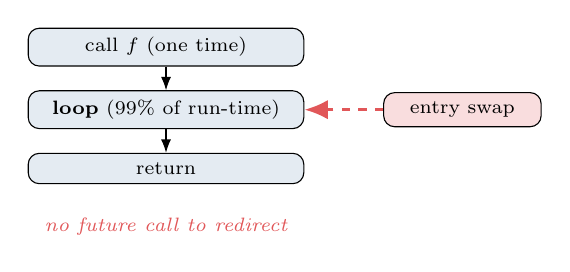
\begin{tikzpicture}[font=\scriptsize,node distance=3mm]
        \node[draw,rounded corners,fill=tier1!15,minimum width=3.5cm] (call) {call $f$ (one time)};
        \node[draw,rounded corners,fill=tier1!15,below=of call,minimum width=3.5cm] (loop) {\textbf{loop} (99\% of run-time)};
        \node[draw,rounded corners,fill=tier2!20,right=10mm of loop,minimum width=2cm] (swap) {entry swap};
        \node[draw,rounded corners,fill=tier1!15,below=of loop,minimum width=3.5cm] (ret) {return};
        \draw[-{Latex}] (call) -- (loop);
        \draw[-{Latex}] (loop) -- (ret);
        \draw[-{Latex[length=3mm,width=2.5mm]},dashed,tier2,very thick] (swap.west) -- (loop.east);
        \node[below=of ret,font=\scriptsize\itshape,color=tier2] {no future call to redirect};
      \end{tikzpicture}
    \end{column}
  \end{columns}
\end{frame}

% ============================================================
\begin{frame}{Three-state back-edge instrumentation}
  Each outermost loop reads one slot of \code{OsrEntryTable} on every back-edge.
  The slot encodes a three-state machine.

  \vspace{0.6em}
  \centering
  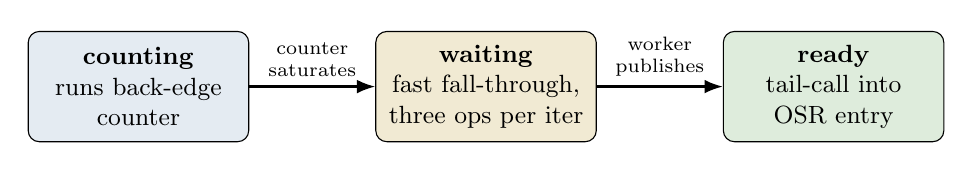
\begin{tikzpicture}[font=\small,
    state/.style={draw,rounded corners,minimum width=2.8cm,minimum height=14mm,align=center}]
    \node[state,fill=tier1!15] (count) {\textbf{counting}\\runs back-edge\\counter};
    \node[state,fill=ntugold!25,right=16mm of count] (wait) {\textbf{waiting}\\fast fall-through,\\three ops per iter};
    \node[state,fill=osrcol!20,right=16mm of wait] (ready) {\textbf{ready}\\tail-call into\\OSR entry};
    \draw[-{Latex},thick] (count) -- node[above,font=\scriptsize,align=center]{counter\\saturates} (wait);
    \draw[-{Latex},thick] (wait) -- node[above,font=\scriptsize,align=center]{worker\\publishes} (ready);
  \end{tikzpicture}

  \vspace{0.8em}
  \textbf{Steady-state cost.} Three operations per iteration in the \emph{waiting} state. An earlier two-array design needed six.
  Full pseudocode in the backup slides.
\end{frame}

\begin{frame}{OSR continuation entry synthesis}
  \textbf{The continuation reuses the mini-module mechanism with three changes.}
  \begin{enumerate}\setlength{\itemsep}{3pt}
    \item \textbf{Parameter list.} The new function takes the original parameters and the original locals, flattened into one list. The caller passes the running frame's state in through the call.
    \item \textbf{Function body.} The body opens the enclosing control constructs, then resumes the original instruction stream from the loop header.
    \item \textbf{Fresh function slot.} The continuation lives in a new slot. The original function stays untouched. Calls inside the continuation dispatch back to the original through \code{t1\_thunk}.
  \end{enumerate}
  \vspace{0.4em}
  \begin{alertblock}{Structural bail-out}
    Some loops cannot be safely re-entered mid-execution. The synthesis rejects those loops and the \tone{} path keeps running them correctly.
  \end{alertblock}
\end{frame}

\begin{frame}{Why OSR continuations drain first}
  \textbf{Two queues share one worker. The OSR queue has priority.}
  \begin{itemize}\setlength{\itemsep}{2pt}
    \item A \ttwo{} batch redirects \emph{future} calls. Late publication still helps.
    \item An OSR continuation migrates a \emph{currently-running} frame.\\
      The migration window closes when the running loop exits.
    \item An OSR continuation that lands after the loop returns is a no-op.
  \end{itemize}
  \vspace{0.6em}
  \textbf{Function-entry promotion and OSR operate independently.}
  \begin{itemize}\setlength{\itemsep}{2pt}
    \item The two mechanisms target different invocation shapes.
    \item One function may be entry-promoted to \ttwo{} \emph{and} carry OSR continuations for its loops at the same time.
  \end{itemize}
\end{frame}

% ============================================================
\section{Evaluation}
% ============================================================

\begin{frame}{Methodology}
  \small
  \textbf{Benchmark suite: sightglass-strong.}\\
  Upstream sightglass kernels run in well under a second.
  The strengthened suite extends each kernel's \tone{}-only run-time into a 5--10\,s band.
  \ttwo{} now has enough post-switch runway to amortize the worker's compile cost.

  \vspace{0.4em}
  \textbf{39 analyzed kernels group into five execution shapes.}
  \begin{itemize}\setlength{\itemsep}{1pt}
    \item \textbf{Frequent-call} (17): one hot function called many times.
    \item \textbf{Hot-leaf} (6): a small helper is called many times and becomes hot before the hot caller.
    \item \textbf{One-shot-caller} (7): outer function called once, dominated by one loop.
    \item \textbf{Resistant} (4): too little run-time or no inline opportunity.
    \item \textbf{Compile-dominated} (7): LLVM compile cost dwarfs the wasm work.
  \end{itemize}
  \vspace{0.3em}
  \textbf{Baselines.} Whole-module LLVM JIT for the throughput ceiling; \tone{} alone for the latency floor.\\
  \textbf{Metrics.} Work-time, compile time, end-to-end wall-clock.
\end{frame}

\begin{frame}{Three configurations, three steps}
  Each step turns on one mechanism on top of the previous step.

  \vspace{0.5em}
  \centering
  \small
  \begin{tabular}{lccl}
    \toprule
    Step & \code{t1/t2} & \code{LLVM/t2} & Mechanism added \\
    \midrule
    Step 1 -- promote hot callees only           & 0.97$\times$ & 0.76$\times$ & function-entry promotion \\
    Step 2 -- walk-up + bounded BFS              & 1.03$\times$ & 0.80$\times$ & better batch composition  \\
    Step 3 -- on-stack replacement (full system) & \textbf{1.11$\times$} & \textbf{0.86$\times$} & in-flight migration \\
    \bottomrule
  \end{tabular}

  \vspace{0.8em}
  \begin{itemize}\setlength{\itemsep}{2pt}
    \item Geometric mean across all 39 kernels.
    \item \code{t1/t2}: how much faster the full system runs than \tone{} alone.
    \item \code{LLVM/t2}: how close the full system gets to whole-module LLVM JIT.\\
      A value of 0.86$\times$ means the full system recovers 86\% of LLVM throughput.
  \end{itemize}
\end{frame}

\begin{frame}{Step 2: walk-up rescues hot-leaf kernels}
  Step 1 batched only the leaf that tripped the counter.
  The optimizer had nothing big enough to inline into.
  Step 2 rolls the surrounding caller into the batch.

  \vspace{0.4em}
  \centering
  \small
  \begin{tabular}{lccc}
    \toprule
    Kernel & Step 1 \code{LLVM/t2} & Step 2 \code{LLVM/t2} & swing \\
    \midrule
    \code{hashset}          & 0.62$\times$ & 0.84$\times$ & +0.22 \\
    \code{shootout-ed25519} & 0.38$\times$ & 0.58$\times$ & +0.20 \\
    \code{rust-json}        & 0.62$\times$ & 0.75$\times$ & +0.13 \\
    \code{rust-compression} & 0.75$\times$ & 0.87$\times$ & +0.12 \\
    \code{regex}            & 0.85$\times$ & 0.95$\times$ & +0.10 \\
    \code{pulldown-cmark}   & 0.75$\times$ & 0.84$\times$ & +0.09 \\
    \code{gcc-loops}        & 0.74$\times$ & 0.83$\times$ & +0.09 \\
    \bottomrule
  \end{tabular}

  \vspace{0.4em}
  \scriptsize
  \textbf{Two groups still lag after Step 2.}
  One-shot-caller kernels (\code{shootout-ctype} 0.37$\times$, \code{blind-sig} 0.40$\times$) need OSR.
  Compile-dominated kernels have flat steady-state; end-to-end wall-clock is the right metric for them.
\end{frame}

\begin{frame}{Step 3: OSR closes the one-shot-caller gap}
  The seven kernels with the largest Step\,2 $\to$ Step\,3 jump all sit in the one-shot-caller group.

  \vspace{0.4em}
  \centering
  \small
  \begin{tabular}{lccc}
    \toprule
    Kernel & Step 2 \code{LLVM/t2} & Step 3 \code{LLVM/t2} & swing \\
    \midrule
    \code{shootout-ctype}     & 0.37$\times$ & \textbf{0.88$\times$} & +0.51 \\
    \code{blind-sig}          & 0.40$\times$ & \textbf{0.80$\times$} & +0.40 \\
    \code{shootout-random}    & 0.63$\times$ & 1.00$\times$ & +0.37 \\
    \code{shootout-base64}    & 0.78$\times$ & 0.99$\times$ & +0.21 \\
    \code{shootout-matrix}    & 0.75$\times$ & 0.95$\times$ & +0.20 \\
    \code{shootout-ratelimit} & 0.79$\times$ & 0.96$\times$ & +0.17 \\
    \code{shootout-minicsv}   & 0.79$\times$ & 0.95$\times$ & +0.16 \\
    \bottomrule
  \end{tabular}

  \vspace{0.4em}
  \textbf{What happens at the swing.}
  The loop's back-edge counter saturates while the loop is still running.
  The worker compiles a continuation.
  The next iteration tail-calls into LLVM-optimized code.
\end{frame}

\begin{frame}{Compile time and end-to-end wall-clock}
  \textbf{Compile time.} How long the runtime spends compiling before steady state.\\
  \textbf{End-to-end wall-clock.} How long the user actually waits.

  \vspace{0.5em}
  \begin{columns}[T,onlytextwidth]
    \begin{column}{0.48\textwidth}
      \begin{block}{Compile-time gain}
        Geometric mean: \textbf{11.1$\times$}.\\
        The full system finishes compilation about 11 times faster than whole-module LLVM JIT.\\
        The \ttwo{} optimizer runs on the worker thread, off the user's critical path.
      \end{block}
    \end{column}
    \begin{column}{0.48\textwidth}
      \begin{block}{End-to-end gain}
        Geometric mean: \textbf{1.73$\times$}.\\
        The full system finishes the end-to-end workload about 73\% faster on average.\\
        The gain comes from saved compile time, even though steady-state throughput is 14\% lower.
      \end{block}
    \end{column}
  \end{columns}
\end{frame}

\begin{frame}{The largest wall-clock wins}
  The wall-clock benefit is largest on compile-dominated workloads.
  These workloads are the real-world targets for the architecture.

  \vspace{0.4em}
  \centering
  \small
  \begin{tabular}{lrrl}
    \toprule
    Kernel & \ttwo{} time & LLVM time & speedup \\
    \midrule
    \code{tinygo-json}                     & 473\,ms   & 10\,361\,ms & \textbf{21.9$\times$} \\
    \code{tract-onnx-image-classification} & 9.7\,s    & 136\,s      & \textbf{14.1$\times$} \\
    \code{spidermonkey-json}               & $\sim$9\,s & $\sim$90\,s & $\sim$10$\times$ \\
    \code{spidermonkey-markdown}           & $\sim$9\,s & $\sim$90\,s & $\sim$10$\times$ \\
    \code{spidermonkey-regex}              & $\sim$9\,s & $\sim$90\,s & $\sim$10$\times$ \\
    \code{image-classification}            & 303\,ms   & 2\,667\,ms  & \textbf{8.8$\times$}  \\
    \code{sqlite3}                         & 1\,985\,ms & 16\,953\,ms & \textbf{8.5$\times$}  \\
    \bottomrule
  \end{tabular}

  \vspace{0.4em}
  \scriptsize
  \textbf{Why the wins cluster here.}
  Each module is interpreter-shaped, reflection-heavy, host-bound, or dominated by large tensor operators.
  The source-to-wasm toolchain has already baked in the hot path, so LLVM cannot recover further speedup.
  Saving the LLVM compile cost is therefore pure win.
\end{frame}

\begin{frame}{Where the tiered design loses ground}
  \textbf{Long-running synthetic kernels.}
  The \tone{} throughput gap is no longer offset by a meaningful cold-start saving.

  \vspace{0.5em}
  \centering
  \small
  \begin{tabular}{lr}
    \toprule
    Kernel & end-to-end vs.\ LLVM \\
    \midrule
    \code{shootout-ctype} & 0.93$\times$ \\
    \code{shootout-sieve} & 0.84$\times$ \\
    \code{shootout-fib2}  & 0.90$\times$ \\
    \bottomrule
  \end{tabular}

  \vspace{0.7em}
  \textbf{The central observation.}
  Workloads split bimodally.
  Compile-dominated workloads win big.
  Long-running synthetic kernels lose a small amount.
  The architecture trades a modest steady-state cost for a large cold-start saving.
  The trade pays off most clearly on the real-world workloads the architecture targets.
\end{frame}

% ============================================================
\section{Limitations and Future Work}
% ============================================================

\begin{frame}{Limitations}
  \begin{description}\setlength{\itemsep}{0.5em}
    \item[No SIMD lowering.]
      \tone{} does not lower wasm SIMD instructions.
      The translator rejects modules that use them.
      The \ttwo{} promotion gate accepts only scalar signatures.
    \item[No de-tiering.]
      Promotion is one-way.
      A function promoted under one workload shape stays promoted even if the shape changes.
    \item[x86-64 only.]
      The current prototype runs on x86-64.
      The library backend supports aarch64, but no aarch64 port has been validated.
    \item[Worker contention on small hosts.]
      The evaluation used a 24-core workstation.
      On a single-vCPU edge node, the worker competes with user code and erodes the wall-clock gain.
  \end{description}
\end{frame}

\begin{frame}{Future work}
  \begin{description}\setlength{\itemsep}{0.6em}
    \item[SIMD lowering and wider promotion scope.]
      Add SIMD lowering to \tone{}.
      Widen the OSR transition buffer for 128-bit slots.
      Relax the promotion gate to admit SIMD and reference-type signatures.
    \item[aarch64 port.]
      Re-derive the bridge thunks for the AArch64 calling convention.
      Re-validate OSR continuation entry parameter layout against the aarch64 register allocator.
    \item[Refcounted JIT cache for de-tiering.]
      Hold \tone{} code alive while a frame may still reach it.
      A function promoted under one workload shape could revert to \tone{} and re-promote later.
    \item[Profile-guided batch policy.]
      Replace the fixed walk-up depth and BFS bound.
      Use call-site frequencies, branch biases, and value profiles to shape each batch.
  \end{description}
\end{frame}

% ============================================================
\section{Conclusion}
% ============================================================

\begin{frame}{Summary}
  \footnotesize
  This thesis presents a \textbf{tiered compilation architecture for WasmEdge} that separates cold-start latency from peak code quality.

  \vspace{0.3em}
  \textbf{Three design components.}
  \begin{itemize}\setlength{\itemsep}{1pt}
    \item \tone{}: Sea-of-Nodes baseline JIT with embedded counters and a uniform calling convention.
    \item \ttwo{}: mini-module synthesis drives the LLVM frontend; three ABI bridge thunks; walk-up batch policy.
    \item \osr{}: three-state back-edge diamond; continuation resumes a running frame mid-loop.
  \end{itemize}

  \vspace{0.3em}
  \textbf{Headline results across 39 kernels.}
  \begin{itemize}\setlength{\itemsep}{1pt}
    \item Compile time: \textbf{11.1$\times$} faster than whole-module LLVM JIT.
    \item Steady-state throughput: \textbf{86\%} of LLVM JIT preserved.
    \item End-to-end wall-clock: \textbf{1.73$\times$} faster on average; up to 21.9$\times$ on \code{tinygo-json}.
    \item OSR closes the one-shot-caller gap: \code{shootout-ctype} 0.37$\times$ $\to$ 0.88$\times$.
  \end{itemize}
\end{frame}

\begin{frame}[plain]
  \centering
  \vfill
  {\Huge\bfseries\color{nturoyal} Thank You}\\[1em]
  {\Large Questions?}\\[2em]
  \begin{tabular}{rl}
    \textbf{Author:}   & Hsiang-Yu Lee (李祥宇) \\
    \textbf{Advisor:}  & Prof.\ Shih-Wei Liao \\
    \textbf{Code:}     & WasmEdge fork with tiered JIT \\
  \end{tabular}
  \vfill
\end{frame}

% ============================================================
% Backup slides
% ============================================================

\appendix

\begin{frame}{Backup: workload categorization (39 kernels)}
  \scriptsize
  \begin{description}\setlength{\itemsep}{3pt}
    \item[Frequent-call (17)] \code{blake3-scalar, bz2, gcc-loops, hashset, pulldown-cmark, quicksort, regex, shootout-gimli, shootout-heapsort, shootout-keccak, shootout-memmove, shootout-seqhash, shootout-sieve, shootout-switch, shootout-xblabla20, shootout-xchacha20, tinygo-regex}
    \item[Hot-leaf (6)] \code{blind-sig, rust-compression, rust-json, rust-protobuf, shootout-ctype, shootout-ed25519}
    \item[One-shot-caller (7)] \code{blind-sig, shootout-base64, shootout-ctype, shootout-matrix, shootout-minicsv, shootout-random, shootout-ratelimit}
    \item[Resistant (4)] \code{richards, rust-html-rewriter, shootout-fib2, shootout-nestedloop}
    \item[Compile-dominated (7)] \code{image-classification, spidermonkey-json, spidermonkey-markdown, spidermonkey-regex, sqlite3, tinygo-json, tract-onnx-image-classification}
  \end{description}
  \vspace{0.3em}
  \code{shootout-ctype} and \code{blind-sig} sit in two groups. Both mechanisms must fire to close the gap.
\end{frame}

\begin{frame}{Backup: why default returns instead of trap stubs}
  \textbf{The earlier design used trap stubs inside the mini-module.}
  LLVM responded in three steps:
  \begin{itemize}\setlength{\itemsep}{2pt}
    \item LLVM marked each trap stub as non-returning.
    \item LLVM folded every call site that referenced a stub into a trap.
    \item LLVM deleted the dispatch path the post-processing pass needed to rewrite.
  \end{itemize}
  \vspace{0.5em}
  \textbf{Default returns avoid the chain.}
  \begin{itemize}\setlength{\itemsep}{2pt}
    \item Each stub returns the function's declared type. Validation succeeds.
    \item Post-processing rewrites the stubs into \code{t1\_thunk}s before the optimizer runs. The call sites survive.
  \end{itemize}
\end{frame}

\begin{frame}{Backup: scope of \texttt{JitExecEnv} writes}
  \textbf{Field ownership keeps cross-thread synchronization simple.}
  \begin{itemize}\setlength{\itemsep}{2pt}
    \item The user thread writes every field except the \code{OsrEntryTable} pointer.
    \item The worker thread writes only the \code{OsrEntryTable} pointer.
    \item Publishing a \ttwo{} batch is one atomic store into \code{FuncTable[i]}.
    \item Publishing an OSR continuation is one atomic store into \code{OsrEntryTable[id]}.
  \end{itemize}
  \vspace{0.5em}
  No locks sit on the hot dispatch path.
  On the supported host architecture, the dispatch load already provides the ordering the design needs.
\end{frame}

\begin{frame}[fragile]{Backup: full pseudocode of the back-edge diamond}
\begin{lstlisting}[language=C]
slot = LOAD OsrEntryTable[loopId]
if slot != WAITING:                  // sentinel 0
  if slot == COUNTING:               // sentinel 1
    counter = LOAD BackEdgeCounters[loopId]
    if counter < threshold:          // unsigned!
      counter += 1
      STORE BackEdgeCounters[loopId] = counter
      if counter == threshold: notify_osr(loopId)
  else:                              // READY: slot holds an entry pointer
    snapshot wasm locals into per-thread buffer
    return slot(env, locals)         // tail-call the OSR entry
fall through to the back-edge
\end{lstlisting}
  The unsigned comparison matters.
  A signed comparison would treat the saturated value as negative and let the gate pass.
  The counter would wrap and re-fire notification on every threshold-th invocation.
\end{frame}

\begin{frame}{Backup: threats to validity}
  \small
  \begin{itemize}\setlength{\itemsep}{3pt}
    \item \textbf{Single-host measurement.}
      All numbers from one 24-core workstation.
      Behavior on production edge hosts is not measured.
    \item \textbf{No CPU contention scenario.}
      The worker thread runs on a dedicated core in the experiments.
      Single-vCPU contention is acknowledged in the limitations but not measured.
    \item \textbf{Sightglass-strong, not cross-runtime.}
      The suite compares successive configurations of one runtime.
      No cross-runtime claim is made.
    \item \textbf{x86-64 only.}
      The aarch64 port is not validated.
  \end{itemize}
\end{frame}

\begin{frame}{Backup: OSR lineage}
  \small
  \textbf{HotSpot pattern.}
  A per-method back-edge counter triggers an OSR compile.
  The OSR compile emits a method version whose entry point is the loop header.
  Live state transfer uses a stack map.
  HotSpot has supported OSR for over two decades.

  \vspace{0.4em}
  \textbf{.NET 7 (2022).}
  Added OSR with the same one-shot-caller motivation this thesis targets.
  The release notes describe methods called once that spend their run-time inside loops.

  \vspace{0.4em}
  \textbf{This thesis.}
  Follows the HotSpot and .NET-7 lineage. Three simplifications:
  \begin{itemize}\setlength{\itemsep}{1pt}
    \item Restricted to outermost-loop back-edges.
    \item Live state is the wasm-level local set, not a stack map.
    \item Continuation is a fresh wasm function compiled through the LLVM frontend.
  \end{itemize}
  WebAssembly's structured control flow makes the simplifications safe.
\end{frame}

\begin{frame}{Backup: why dstogov/ir, not Cranelift}
  \small
  \textbf{Three reasons dstogov/ir fits the baseline tier role.}
  \begin{itemize}\setlength{\itemsep}{3pt}
    \item \textbf{Bounded, predictable compile latency.}
      The library runs a fixed, linear pipeline with no pass manager.
      Compile cost scales linearly with function size.
    \item \textbf{SSA-quality output from a single-pass frontend.}
      The IR is SSA by construction.
      The thesis does not need a separate SSA-construction phase.
    \item \textbf{Small enough to vendor and modify.}
      The runtime can extend the library when a backend change is needed.
  \end{itemize}

  \vspace{0.4em}
  \textbf{Why not Cranelift.}
  Cranelift's pipeline targets higher code quality at higher compile cost.
  Cranelift is closer to an optimizing tier than a baseline tier.
  The codebase is also larger and harder to vendor.
\end{frame}

\begin{frame}{Backup: bibliography highlights}
  \footnotesize
  \begin{itemize}\setlength{\itemsep}{2pt}
    \item Click \& Paleczny, \emph{A simple graph-based intermediate representation}, IR '95. -- Sea-of-Nodes.
    \item Click, \emph{Global code motion / global value numbering}, SIGPLAN '95.
    \item Fink \& Qian, \emph{Adaptive recompilation with on-stack replacement}, CGO 2003.
    \item D'Elia \& Demetrescu, \emph{On-stack replacement, distilled}, TOPLAS 2018.
    \item Bytecode Alliance, \emph{Wasmtime baseline compilation RFC}, 2022.
    \item Clark, \emph{Firefox's streaming and tiering compiler}, Mozilla Hacks, 2018.
    \item Chen et al., \emph{Accelerate RISC-V instruction set simulation by tiered JIT compilation}, VMIL 2024.
    \item Stogov, \emph{dstogov/ir}: Sea-of-Nodes JIT library.
  \end{itemize}
\end{frame}

\end{document}
